\documentclass[main.tex]{subfiles}
\begin{document}
\chapter{Background}\label{chap:Background}
In this chapter, we present relevant literature needed to completely understand the proposed concept of \autoref{chap:Concept}.

\section{SLAM}
SLAM (Simultaneous Localization And Mapping) algorithms aim to solve a usual problem in the field of unmanned robotics;
A robot finds itself in an unknown environment and attempts to build a coherent map while keeping track of its location.
The robot uses use-case-specific sensors to obtain a snapshot of its current surroundings, which it then uses to update and enhance its known map (Mapping).
The robot simultaneously attempts to accurately estimate its position based on the updated map ($Localization$).
The new information about its position is processed during the next map update.

Over decades of research, varieties of different (combinations of) sensors have been employed to solve this problem more accurately and efficiently.
Internal odometry sensors alone can be unreliable if the robot moves over uneven or slippery surfaces.
Visual sensors are, therefore, integrated into many SLAM methods, making them a Visual-SLAM (VSLAM) method. Therein, the methods can be
further divided into \textit{visual-only, visual-intertial}, and \textit{RGB-D} SLAM~\cite{vslamsurvey}.

\textit{Visual-only} SLAM algorithms are solely based on the input of a camera.
Popular VSLAM algorithms include \textit{ORB-SLAM2}~\cite{Mur-Artal_Tardós_2017}, $MonoSLAM$~\cite{davison2007monoslam},
and DSO-SLAM~\cite{engel2017direct}.

\textit{Visual-intertial} SLAM methods integrate additional sensor information from an \textit{Inertial Measurement Unit} (IMU).
The IMU provides information about the rotation, acceleration, and magnetic field around the device. These types of information
generally aid the estimations based on visual input. However, the IMU data needs additional estimations,
which increases the SLAM's complexity. \textit{ORBSLAM3}~\cite{campos2021orb} and \textit{Robust Visual Inertial Odometry} (ROVIO)~\cite{bloesch2017iterated}
are \textit{visual-intertial}-based SLAM methods.

Lastly, RGB-D SLAM methods combine a monocular RGB camera and a depth sensor. This combination removes additional calculations
initially needed to obtain depth information. \textit{Dense Visual Odometry} (DVO)~\cite{Kerl_Sturm_Cremers_2013} and $RGBDSLAMv2$~\cite{endres20133} are instances of
popular RGB-D SLAM methods.

% FIXME top-level Diagram!



\subsection*{Real-Time Appearance-Based Mapping}
% RealSense-ROS internally uses a SLAM algorithm for map building, namely RTAB-MAP (Real-Time Appearance-Based Mapping)\cite{Labbé_Michaud_2019}.
Real-Time Appearance-Based Mapping (RTAB-MAP) is a $VSLAM$ system with an optional IMU input, making it a \textit{visual-intertial} SLAM.
RTAB-MAP's general workflow is shown in Figure~\ref{fig:rtabmap}.
All these inputs are combined during a synchronization step, and the results thereof are passed to RTAB-MAP's Short-Term-Memory (STM).
The STM assembles a new node from the new inputs and inserts it into the map graph. Based on the newly inserted node, RTAB-MAP attempts to
determine if the current location has already been visited earlier, also known as \textit{loop closure}.
If a loop closure is detected, i.e., RTAB-MAP detects the re-visiting of a known location, the map graph is optimized and thus minimized.
In addition, the global map is reassembled in correspondence with the new information.
The resulting map is published in the form of an \textit{unorganized point cloud} (see Subsection~\ref{subsec:input}).

\begin{figure}[!h]
    \centering
    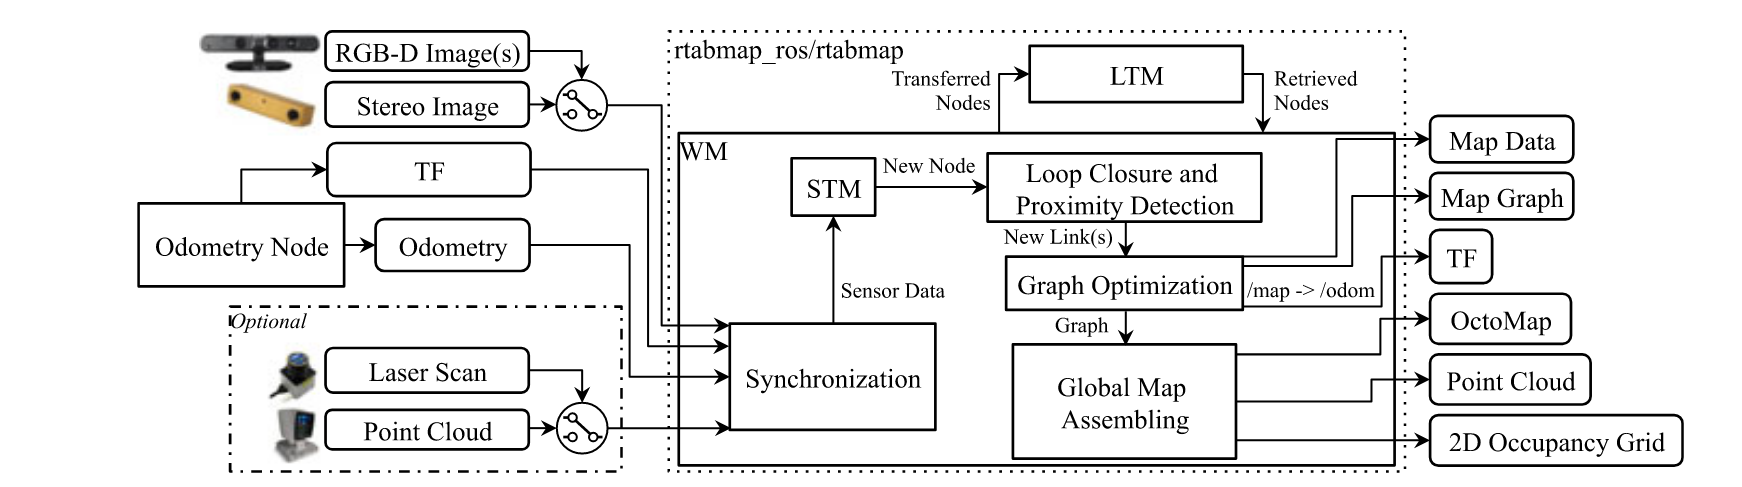
\includegraphics[width=15 cm]{images/rtabmap.png}
    \caption[RTAB-MAP Block Diagram]{Block diagram of RTAB-MAP's system architecture. Note, that the \textit{Point Cloud} returned by the \textit{Global Map Assembling}
        is an unorganized point cloud (see Section~\ref{sec:dataformats}).
        Taken from \cite[Figure~1]{Labbé_Michaud_2019}}
    \label{fig:rtabmap}
\end{figure}

\section{Intel Realsense}
In this work, we use the Intel RealSense tracking camera T265 and the RGB-Depth(RGB-D) camera D455.
A tracking camera is generally used to observe the environment and usually has a wider field of view (FOV). The primary motivation for using RGB-D cameras is depth perception.
The primary differences and similarities between the T265 and the D455 are reported in Table~\ref{tab:cameraspecs}.
Beide Kameras sind stereo, die T265 hat 2 fisheye lenses und die D455 hat 2 imagers. Dazu hat die D455 noch einen RGB sensor und einen infrarot sensor. Mit dem IR sensor und den beiden imagern wird ein tiefenbild berechnet.
Durch die fisheye lenses hat die T265 mit 163° ein deutlich breiteres Sichtfeld  als die D455 mit nur 111°. Die maximale FPS anzahl der D455 ergibt sich aus den individuellen FPS werten der imager sensoren und dem RGB sensor, welche beide einen maximalwert von 90 haben.
Dazu sei gesagt, dass bei steigender auflösung die maximale Framerate sinkt und 90FPS nur mit einer maximalen auflösung von 640x480 möglich ist.
Furthermore, both cameras have an integrated Inertial Measurement Unit (IMU) which is used to compute its position in combination with visual input.
% FIXME explain tracking and RGB-D

Intel provides a software development kit, namely RealSense SDK, which allows easy and efficient use of the cameras.
The SDK runs on both Windows and Ubuntu, and a ROS(Robot Operating System \footnote{\href{https://www.ros.org/}{https://www.ros.org/}}) adaptation is also provided in Intel's Github repository \footnote{\href{https://github.com/IntelRealSense/realsense-ros}{https://github.com/IntelRealSense/realsense-ros}}.

\begin{table}[H]
    \centering
    \begin{tabular}{c|ccccccc}
             & Image  & Type     & max. Resolution & D-FOV & Shutter & Price & max. FPS \\ \hline
        D455 & Stereo & RGB-D    & 1280x720        & 111°  & global  & 419\$ & 90       \\ \hline
        T265 & Stereo & Tracking & 848 x 800       & 163°  & global  & 199\$ & 30
    \end{tabular}
    \caption[Intel RealSense T265 & D455 Specification]{Intel RealSense T265 and D455 camera specifications. More information and the complete Datasheets can be found on https://www.intelrealsense.com/.}
    \label{tab:cameraspecs}
\end{table}


\section{Data Formats}
\label{sec:dataformats}
In the following chapters, we often refer to different data representations, namely the data that is given into a plane detection algorithm, and
the exportation format of the planes. The following subsections provide necessary information and further distinctions.


\subsection{Common Input Types}
\label{subsec:input}
Usually, the data representation of the recorded environment falls into one of three categories:
\begin{itemize}
    \item \textit{unorganized} or \textit{unstructured point cloud} (UPC)
    \item \textit{organized} or \textit{structured point cloud} (OPC)
    \item image:
          \begin{itemize}
              \item Depth (DI)
              \item RGB (RGBI)
          \end{itemize}
\end{itemize}

The input types are compared in Table~\ref{tab:inputs}. Both the organized and the unorganized point cloud store 3D coordinates.
The fundamental difference between UPC and OPC is their format,
In the popular point-cloud-library (PCL) data format\footnote{\href{http://pointclouds.org/documentation/tutorials/pcd\_file\_format}{http://pointclouds.org/documentation/tutorials/pcd\_file\_format}},
each point cloud has a \textit{width} and a \textit{height}.
The \textit{width} of a UPC is the number of included points, while the \textit{height} equals 1.
In contrast, the \textit{width} and \textit{height} of an OPC depend on the resolution of the recording camera.
For instance, recording the environment with an arbitrary camera with a resolution of 640x480, each organized point cloud
would have a \textit{width} and \textit{height} of $640$ and $480$, respectively. Another distinguishing factor is that the organized
point cloud can only represent the environment from one angle, which leads to missing data due to sensor limitations and the occlusion
of points that lie behind other points. Conversely, UPCs are neither limited to a specific viewport nor do they allow for missing points.

When considering images, a differentiation between RGB images and depth images has to be made.
Depth mages are inherently similar to organized point clouds, given their resolution and two-dimensional structure.
The primary difference is that the matrix stores distances to the sensor instead of 3D coordinates.
RGB images are, like Depth images, stored as a 2D Matrix but instead of distances or coordinates, the matrix stores
values that describe the color of a pixel. Usually, this means that each pixel stores a triple that describes a specific
color by the amount of included red, green, and blue.

\begin{table}[H]
    \centering
    \begin{tabular}{c|c|c|c}
        \textbf{Input Type} & \textbf{Value Types} & \textbf{Memory Layout} & \textbf{0 or NaN} \\ \hline
        \textbf{OPC}        & 3D Coordinates       & 2D Matrix              & N                 \\
        \textbf{UPC}        & 3D Coordinates       & 1D Array               & Y                 \\
        \textbf{DI}         & Distances to Sensor  & 2D Matrix              & Y                 \\
        \textbf{RGBI}       & RGB                  & 2D Matrix              & Y
    \end{tabular}
    \caption{Possible inputs for plane detection algorithms columns dedicated to the stored data, the memory layout, and whether
        the input type allows for invalid values.}
    \label{tab:inputs}
\end{table}
It is worth noting that, in the literature, the terms "depth image", "depth map" and "organized point cloud" are used interchangeably.

\textbf{\textcolor{red}{lidar?}}

\subsection{Common Output Formats}
\label{subsec:output}
The format of the detected planes has to conform to the specific application. For instance, an architectural remodeling application
would require the output to be able to contain non-rectangular shapes and holes.
An algorithm that returns a set of planes represented by their convex hull would not be appropriate because it
would fail to correctly represent planes like the top of a corner desk or a wall with a doorway.

Being related to the input format, the output of plane detection algorithms can be clustered as follows:
\begin{itemize}
    \item The cartesian plane equation parameterized by its normal vector and/or its distance to the origin ($n/+d$), \textit{and}
    \item Plane inliers:
          \begin{itemize}
              \item $3D$ inliers (3D-IN), $or$
              \item $2D$ inliers (2D-IN).
          \end{itemize}
\end{itemize}

A common output format is a plane parameterized by its normal vector $n$ and its distance to the origin $d$. This representation
describes a plane as infinitely dense and unbound, if no further information is provided, e.g. extents in certain directions.

We differentiate between the plane inliers according to the way, individual values are accessed.
3D inliers are a set of 3D coordinates that represent a plane in an unorganized point cloud. Like the point cloud itself,
the inliers are accessed through their 1D index within the set.
In contrast, 2D inliers are a set of indices that correspond to values in an organized point cloud, depth image, or RGB image.
Moreover, some methods return a set of segmentation masks, which we also refer to as 2D inliers.
Note, that we include organized point clouds in the 2D case of inliers even though the values inside are three-dimensional,
as the access thereof is still grid-like.

\section{Plane Detection}
The field of plane detection has been around for decades.
Most methods of detecting planar regions in unorganized point clouds are based on one of three main categories \cite{LimbergerOliveira2015HT3D, Araújo_Oliveira_2020}:
\begin{itemize}
    \item Hough Transform (HT)
    \item RANSAC (RC)
    \item Region Growing (RG)
\end{itemize}

\subsection{Hough Transform}
The original motivation behind the Hough transform was detecting lines in images~\cite{5230799}. All points are sequentially processed via a voting procedure to detect the best-fitting line over a set of 2d points.
Multiple lines with different orientations are fit through each given point $p$.
Because a line in slope-intercept form parallel to the y-axis would lead to an infinite slope, the Hesse normal form is chosen as the primary line representation\cite{10.1145/361237.361242}.

In Hesse normal form, an individual line can be parameterized with a pair $(r, \theta)$, with $r$  being the orthogonal distance origin to the plane and $\theta$ being the angle between the x-axis and the line that connects the origin to the closest point on the line.
This pair is also called a \textit{Hough Space} in this context. Votes are cast on the corresponding value of $\theta$, depending on the number of inliers within a specific \textit{Hough Space} $(r_i,\theta_i)$. The map that connects the
votes to each $\theta$ is called an \textit{accumulator}.
Finally, the best-fitting line is determined by the number of votes it received.

% FIXME besser schreiben
In the context of plane detection in 3D point clouds, a plane would be uniquely identified by the triple $(\rho, \theta, \phi)$, with $\rho$ being the orthogonal distance from the origin to the plane, $\theta$ being the azimuthal angle, and $\phi$ being the inclination.
Since more parameters are needed to describe a plane in 3D, the accumulator must be adapted.
Therefore, a three-dimensional accumulator is used, whereas the specific shape has been discussed~\cite*{Borrmann_Elseberg_Lingemann_Nüchter_2011}.

\subsection{RANSAC}
RANSAC (RAndom SAmple Consensus) has been researched for decades. While many use cases revolve around image processing, it is also heavily employed in many plane detection algorithms\cite{Sun_Mordohai_2019, Yang_Forstner, Ashraf_Ahmed_2017}.
RANSAC is an iterative process. Each iteration randomly samples a certain amount of data points and fits a mathematical model through them. The level of outliers determines the quality of the obtained model and preserves the best overall model.

Within the context of plane detection in 3D point clouds, an approach could involve random sampling of 3 points, fitting a plane through them,
and counting the number of points within a certain range of the plane\cite{Yang_Forstner}. The model, in that case, could be a cartesian plane equation.

\subsection{Region Growing}
Region Growing methods are often used in the field of image or point cloud segmentation \cite{Proença_Gao_2018, Vo_Truong-Hong_Laefer_Bertolotto_2015}.
RG-based segmentation methods aim to grow a set of disjoint regions from an initial selection of seed points. The regions increase in size by inserting neighboring values based on an inclusion criterion.
The quality of the resulting regions depends on the choice of seed points, e.g., a very noisy seed point could decrease overall quality  \cite{Malek_Rahman_Yasiran_Jumaat_Jalil_2012}.
In the context of this work, a criterion for region growth could be the distance or curvature between a region and its adjacent data points.

\section{Plane Detection Algorithms}
The following subsections detail the necessary background knowledge of all the plane detection algorithms mentioned in this paper.
Aside from the functionality of a method, we give relevant higher-level information, e.g., the expected input format and the proposed output format.

\subsection{Robust Statistics approach for Plane Detection}
\label{subsec:bg-rspd}


Robust Statistics approach for Plane Detection (RSPD)~\cite{Araújo_Oliveira_2020} is based on region growing.
After taking an unorganized point cloud as input, the procedure is divided into three phases:
\textit{Split, Grow and Merge} (see Figure~\ref{fig:rspd}).

\paragraph{Split}
The authors propose to use an octree to recursively subdivide the point cloud. 
The subdivision is repeated until every leaf node contains less than a threshold $\varepsilon$ corresponding to the 
minimum number of points per leaf. The authors propose a value of $\varepsilon = 0.1\%$. Alternatively, the subdivision terminates
if a node reaches the maximum depth level $l_O = 10$. Note, that this parameter is not referenced in~\cite{Araújo_Oliveira_2020}. 
However, it is used in the official implementation\footnote{\href{keyhttps://github.com/abnerrjo/PlaneDetection}{https://github.com/abnerrjo/PlaneDetection}}.
The subdivision is followed by a planarity test~\cite[Section~3.2]{Araújo_Oliveira_2020}, during which the octree is traversed bottom-up. 
If all eight children of a node $n$ are leaf nodes and fail the planarity test, $n$ replaces its children
and becomes a leaf node of its own. This procedure is repeated until the root of the octree is reached.

\paragraph{Grow}
In preparation for the growth phase, a neighborhood graph (NG) over the entire point cloud is created. 
Every node of NG represents one point, and an edge between two nodes exists only if
a nearest-neighbor search with a neighborhood size $k$ detects both points being in the same neighborhood. 
The authors use a neighborhood size of $k=50$.


The graph construction is subsequently followed by a breadth-first-search, during which a point $x$ is inserted into a planar patch $p$ if it satisfies the following conditions:
\begin{itemize}
    \item $x$ is not included in any patch \textit{and}
    \item $x$ satisfies the inlier conditions for $p$: % FIXME explain them !
          \begin{itemize}
              \item The distance $d$ of $x$ to $p$ is smaller than a threshold $\theta_d$ (see Eq.~\ref{eq:incond1}) \textit{and} % TODO MDP
              \item The angle $\phi$ between the normals vectors of $x$ and $p$ is less than a threshold $\theta_a$ (see Eq.~\ref{eq:incond2}). % TODO MND
          \end{itemize}
\end{itemize}

\begin{equation}
    \label{eq:incond1}
    d = |(x - p.center)\cdot p.normal| < \theta_d
\end{equation}
\begin{equation}
    \label{eq:incond2}
    \phi = acos(|x.normal, p.normal|) < \theta_a
\end{equation}

\paragraph*{Merge}
In the last phase, the previously grown patches are merged. Two planar patches $P_1$ and $P_2$ can be merged, if the following conditions are met:
\begin{itemize}
    \item The octree nodes of $P_1$ and $P_2$ are adjacent,
    \item $P_1.n$ and $P_2.n$ have a divergence within a tolerance range \textit{and}
    \item at least one inlier of $P_1$ satisfies the inlier conditions(see Eq.~\ref{eq:incond1}+\ref{eq:incond2}) from $P_2$ and vice versa.
\end{itemize}

This phase returns all maximally merged planar patches, i.e. the final planes.

\begin{figure}[]
    \centering
    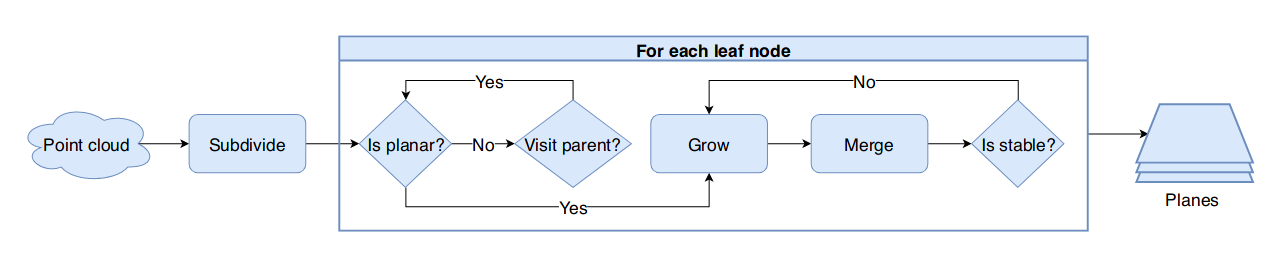
\includegraphics[width=\textwidth]{images/rspd.png}
    \caption[RSPD Pipeline]{The RSPD plane detection pipeline. Taken from~\cite[Figure~2]{Araújo_Oliveira_2020}.}
    \label{fig:rspd}
\end{figure}

\subsection{Oriented Point Sampling}
\label{subsec:bg-ops}
Oriented Point Sampling (OPS)~\cite{Sun_Mordohai_2019} accepts an unorganized point cloud as input.


First, a sample of points is uniformly selected. Sample sizes of $\alpha_s \in [0.3\%,3\%]$ are used in the Evaluation in~\cite[Table~3]{Sun_Mordohai_2019}.
The normal vectors of these points are estimated using SVD and the k nearest neighbors ($KNN$), which are obtained using a k-d tree. 
An inverse distance weight function is employed to prioritize neighboring points that are closer to the sample of which the normal vector is currently being estimated.


After normal estimation, one-point-RANSAC is performed. Usual RANSAC implementations sample three points to fit a plane. 
However, OPS fits a plane with only one sample point and its normal vector and counts the number of points where the distance to
the plane is smaller than a \textit{minimum-distance parameter} $\theta_h$. Moreover, this number of inliers must exceed a 
\textit{minimum plane size} threshold $\theta_N$, for a plane to be accepted.
Once a plane with the most inliers is obtained, its normal vector is re-estimated using SVD on all inliers, and all inliers are removed from the point cloud.
Furthermore, the number of needed iterations $I$ is adaptively determined in each iteration, see Equation~\ref{eq:ops}. 
\begin{equation}
    \label{eq:ops}
    I = \frac{\log(1-p)}{\log(1-(1-e))},
\end{equation}
where $e$ is the ratio of outliers left in the point cloud, and $p$ is a tuneable parameter that corresponds to the likelihood
that a random sample includes no outliers.
This process is repeated until the number of remaining points falls below a predefined threshold $\theta_N$.
After termination, smaller detected planes are merged if they pass a coplanarity test. After a successful merging of planes,
the normal of the resulting plane is calculated via singular value decomposition (SVD).

\subsection{3D Kernel-based Hough Transform}
\label{subsec:bg-3dkht}
With the 3D Kernel-based Hough Transform (3D-KHT),
\citeauthor{LimbergerOliveira2015HT3D}~\cite{LimbergerOliveira2015HT3D} propose a hough transform-based plane detection method,
that accepts unorganized point clouds as input.

The point cloud is spatially subdivided. The authors propose the usage of octrees over k-d trees because the k-d tree lacks efficiency in creation and manipulation.
Furthermore, the octree succeeds in capturing the shapes inside the point cloud, while the k-d tree does not.
The octree level, at which the algorithm starts to check for approximate coplanarity under nodes is adjusted through 
the corresponding parameter $s_{level}$.

Approximate coplanarity of a point cluster is evaluated based on its eigenvalues and two parameters $s_\alpha, s_\beta$.
Therein, $s_\alpha$ corresponds to the tolerance regarding noise, and $s_\beta$ corresponds to the tolerance regarding the 
anisotropy of the included points. The authors report good results with $s_\alpha=25$ and $s_\beta=6$.

Each leaf inside the octree continues subdividing until the points inside a leaf node are considered approximately coplanar, 
or the number of points is smaller than a minimum-points threshold $s_{ps}$.
The authors recommend $s_{ps}=30$ for large point clouds. However, no definition of large in 
this context is given.
After the approximately coplanar nodes are refined by removing outliers, a plane is fit through the remaining points.


This plane $\pi$ can, in polar coordinates, be uniquely described by a triple $(\rho, \theta, \phi)$.
Inspired by \citeauthor{Borrmann_Elseberg_Lingemann_Nüchter_2011}~\cite{Borrmann_Elseberg_Lingemann_Nüchter_2011}, an accumulator ball (Fig.~\ref{fig:accball}) is used for the voting procedure because the cells in polar regions are smaller (and therefore
contain fewer normal vectors) in three-dimensional accumulator arrays, as portrayed in Figure~\ref{fig:accarr}.
Furthermore, the discretization of the accumulator is determined by tuneable parameters, namely $\phi_{num}$ and $\rho_{num}$.
No additional parameter is employed for the discretization of $\rho$, as this is allocated as needed during the voting procedure.
The authors use $\phi_{num}=30$ and $\rho_{num}=300$ during their evaluation.

\begin{figure}[H]
    \centering
    \hspace{\fill}
    \begin{subfigure}{0.25\textwidth}
        \centering
        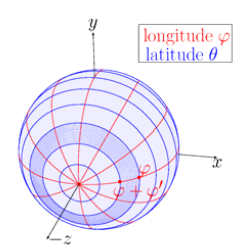
\includegraphics[width=\textwidth]{images/accumulatorarray.png}
        \caption[3D-KHT Accumulator Array]{}
        \label{fig:accarr}
    \end{subfigure}
    \hspace{\fill}
    \begin{subfigure}{0.25\textwidth}
        \centering
        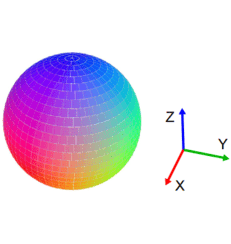
\includegraphics[width=\textwidth]{images/accumulatorball.png}
        \caption[3D-KHT Accumulator Ball]{}
        \label{fig:accball}
    \end{subfigure}
    \hspace{\fill}
    \caption[Hough Transform Accumulators]{Accumulator array (a), taken from \cite*[Figure~3]{Borrmann_Elseberg_Lingemann_Nüchter_2011}. Accumulator
        ball(b) used in 3D-KHT, taken from \cite*[Figure~5]{LimbergerOliveira2015HT3D}.}
\end{figure}

During the voting procedure, votes are not cast for each data point but rather on previously calculated approximately coplanar clusters.
When casting a vote on a given cluster $c_i$ with its plane (represented by $(\rho, \theta, \phi)$), the corresponding entry in the accumulator ball is updated.
With this update, its neighboring clusters also receive a vote determined by the uncertainty value of $c_i$. Due to the non-discrete
values of uncertainty, the votes are floating-point values as well.

All Peaks within the accumulator ball are detected in the last step. Because the votes tend to be sparsely distributed \cite[Section~3.4]{LimbergerOliveira2015HT3D},
an auxiliary array $A$ is used to memorize the entries inside the accumulator that are set. When an accumulator index is assigned a value for the first time, it is also added to $A$.
Therefore, it is only necessary to iterate the auxiliary array to find peaks inside the accumulator.
Furthermore, an intermediary smoothing step is performed by merging adjacent peaks inside the accumulator and storing them in $A$.
Then, $A$ is sorted in descending order.
If a cell $c$ in the accumulator has not yet been visited during iteration, $c$ is considered a peak. In addition, $c$ and its 26 neighboring cells are tagged as \textit{visited}.
That way, the most dominant plane, i.e., the one with the most votes, is detected first.
Finally, the detected planes are sorted by the number of different clusters that voted for them.

\subsection{Octree-based Region Growing}
\label{subsec:bg-obrg}
Octree-Based Region Growing (OBRG) \cite{Vo_Truong-Hong_Laefer_Bertolotto_2015} employs region growing to detect planes in UPC.

First, an unorganized point cloud is recursively subdivided using an octree.
An octree node $n$ repeatedly subdivides itself into eight children until the level of $n$ supersedes a predefined maximum subdivision value or if the
amount of contained points in $n$ is less than a predefined minimum of included points. 
Saliency features are calculated for every leaf node in preparation for the region growing step: A normal vector is obtained by performing a principle
component analysis (PCA) on the points inside each leaf node. The best-fitting plane of each leaf is defined by the mean normal vector and its center point.
A residual value is obtained by taking the root-mean-square (RMS) of the distance of all included points to the plane.

\begin{figure}[H]
    \centering
    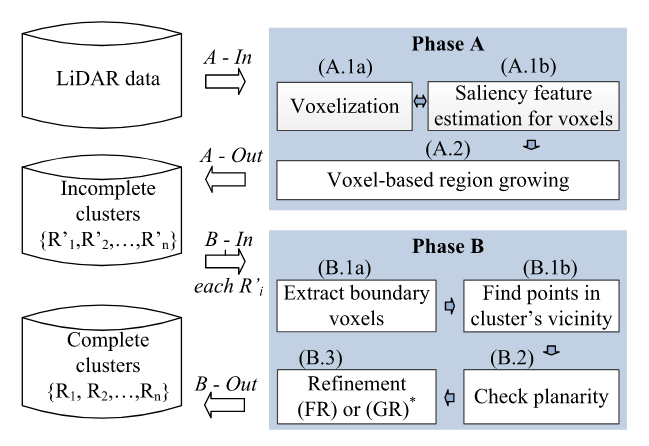
\includegraphics[width=0.7\textwidth]{images/obrg.png}
    \caption[OBRG Pipeline]{The OBRG plane detection pipeline. Taken from~\cite[Figure~1]{Vo_Truong-Hong_Laefer_Bertolotto_2015}.}
    \label{fig:obrg}
\end{figure}

For the region growing phase, all leaf nodes are selected as individual seed points. 
Starting from the seed with the lowest residual value, a neighboring leaf node $n$ is inserted into the region if $n$ 
does not belong to any region and the angular divergence between both normal vectors is smaller than a predefined threshold 
$\theta_{ang}$. Values between $3.5$ degree and $15$ degree were used during the  evaluation~\cite[Tables~1,4,7]{Vo_Truong-Hong_Laefer_Bertolotto_2015}.
Furthermore, if a leaf node is inserted into a region, it is also considered a starting point for a future iteration, 
if its residual value is lower than the corresponding threshold $\theta_{res}$. Small values at a maximum of $0.05$(m)
are reported. If a region cannot be expanded, it is marked as \textit{detected}, if its number of inliers exceeds a 
threshold $\theta_M$.
  
Lastly, a refinement step is employed. 
For efficiency reasons, it is only performed on voxels at the edge of segments.
Fast refinement (FR) is performed on regions that succeed in a planarity test, i.e., 70\%-90\% ($\theta_p$) 
of included points fit the best plane~\cite[Section~3.4]{Vo_Truong-Hong_Laefer_Bertolotto_2015}. 
FR is leaf-based, and all previously unallocated neighboring nodes are added to the region if the point-to-plane distance is smaller 
than a distance threshold $\theta_d$.
General refinement (GR) is performed on regions that are considered non-planar. In contrast to the fast refinement, GR is point based. Therefore,
points from neighboring and previously unallocated leaf nodes are considered and inserted into the region if they, too, satisfy the inlier criterion.
The refinement process returns a complete set of planar regions.

\subsection{Probabilistic Agglomerative Hierarchical Clustering}
\label{subsec:bg-peac}
Probabilistic Agglomerative Hierarchical Clustering (PEAC)~\cite{Feng_Taguchi_Kamat_2014} is a plane detection algorithm that takes an organized
point cloud as input.
The agglomerative hierarchical clustering is based on an algorithm called
\textit{line regression}\cite[Section~III.B]{Nguyen_Martinelli_Tomatis_Siegwart_2005}. The primary difference is
that, instead of a double linked list, PEAC operates on a graph $G$.

First, the input organized point cloud is divided into non-overlapping nodes through the initialization of $G$.
Each node in $G$ has a pre-determined height $H$ and width $W$, whereas $H$ and $W$ correspond to index ranges in the
point cloud, i.e., each node contains a set of points.
Then, $G$ is refined by removing the following types of nodes and corresponding edges~\cite[Section~III.A]{Feng_Taguchi_Kamat_2014}:
\begin{enumerate}
    \item Nodes that contain NaN or 0 values, e.g., missing data,
    \item nodes that contain at least one point that is depth-discontinuous with its four neighbors, e.g., neighbors
          in the pixel space but not in coordinate space,
    \item nodes with a high MSE, e.g., non-planar regions, \textit{and}
    \item nodes that share an edge with two different planes, e.g., the corners of walls.
\end{enumerate}
During this step, all points inside a node share a common plane normal.

The \textit{agglomerative hierarchical clustering} step starts with the construction of a min-MSE-heap data
structure that contains the nodes of $G$, sorted in ascending order by the value of their MSE.
The following steps are then repeated exhaustively.
First, the node $v$ that has the current minimum MSE is merged with one of its neighbors $u$ that minimizes the merged MSE.
If the merged MSE is larger than a threshold $\theta_{MSE}$, then a plane is found and the merged node is removed from G.
if $MSE_{merge}$ is larger than a threshold $\theta_{MSE}$, then a plane segment is found and extracted from $G$.
Otherwise, the merged node is added back to $G$, joining the edges of $v$ and $u$.

Lastly, a refinement step is employed. Due to the clustering of nodes that contain a set of points, certain types of
artifacts can occur:
\begin{itemize}
    \item Sawtooth,
    \item unused data points, \textit{and}
    \item over-segmentation.
\end{itemize}
First, if not all neighbors of a node $v$ belong to the plane of $v$, all points of $v$ are added to a queue $Q_{RG}$.
Then, region growing is performed on the points inside $Q_{RG}$, where the 4-connected neighbors are observed.
A neighboring point $n$ is inserted into the segment $k$ of a point $v$ if $n$ does not belong to $k$, and
the distance to $k$ is smaller than the distance to its current segment. Additionally, $n$ is inserted into $Q_{RG}$,
which also happens if $n \in k$.
The region growing is followed by another \textit{agglomerative hierarchical clustering} step.


\subsection{Fast Cylinder and Plane Extraction}
\label{subsec:bg-cape}
Fast Cylinder and Plane Extraction (CAPE)~\cite{Proença_Gao_2018} is a region growing-based algorithm that detects
planes and cylinders in organized point clouds.
The authors propose this algorithm as an extension of their Probabilistic Visual Odometry Framework~\cite{Proenca_Gao_2018}.

In preparation for the region growing step, the cloud is subdivided into patches of pre-defined size, similar to
the graph initialization of PEAC (see Section~\ref{subsec:bg-peac}).
A patch size of 20x20 was used in their evaluation~\cite[Section~V.A]{Proença_Gao_2018}.
Then, the planarity of the patches is tested, and a patch is considered non-planar, if:
\begin{itemize}
    \item The amount of NaN or 0 points exceeds a threshold, \textit{or}
    \item the patch has depth discontinuities,
\end{itemize}
whereas the depth discontinuities are only checked for pixels on an axis-aligned cross through the center of the patch
A plane is then fit through the patch inliers by performing principle component analysis (PCA). The plane's MSE
corresponds to the lowest eigenvalue, and the plane's normal vector is its eigenvector.
A patch is considered planar, if its mean depth value is within the standard deviation of all depth values in the patch, plus a tolerance.

The normal vectors are converted from cartesian to spherical coordinates, thus being described by a polar angle, and
an azimuth angle. These spherical normal vectors are then assorted into bins, thus building a histogram $H$.
This histogram is now used for the region growing step.
First, a set of patches $C$ of the most frequent bin in $H$ are obtained. Stop, if the most frequent bin
yields fewer patches than a threshold $k_1$. The patch with the smallest MSE out of $C$ is chosen as a seed $s$.
In general, a 4-connected neighborhood is used in this approach, and a neighboring patch $n$ is inserted into a region, if:
\begin{enumerate}
    \item $n$ is not assigned to any region,
    \item the dot product of both patches normal vectors is less than a threshold $T_N$, \textit{and}
    \item the orthogonal distance of $n$'s center to the region is less than $T_d(s) = l\sqrt{(1-T_N^2)}$,
\end{enumerate}
where $l$ is the distance between the corner points of $s$.
If a complete segment $S$ is found, all included patches are removed from the list of remaining patches, and
the bins of the histogram are updated accordingly. Lastly, if $S$ exceeds the minimum plane size $k_2$, it is added
to the set of detected planes.

The planarity of all segments is now assessed. This is done by calculating the covariance of all included points and,
subsequently, comparing the ratio of the second largest eigenvalue to the smallest eigenvalue thereof. If this ratio
exceeds a pre-determined parameter $plane_min_score$, the segment is considered a plane.
Otherwise, additional steps are needed.
First, the surface of a segment is checked for invariance, which is a property of open cylinders.
For this task, PCA is performed on the stacked matrix of normal vectors of the segment.
Then, the ratio of the first eigenvalue to the last eigenvalue of this covariance matrix, namely the condition number,
is calculated. If the condition number exceeds a threshold $\theta_{cond}$, the segment is comprised of a set of
cylinders or planes~\cite[Section~III.D]{Proença_Gao_2018}.

Using the eigenvector with the smallest eigenvalue, the center points and normal vectors of all patches
in the segment are then projected onto a plane. Then, multiple models are fit by performing sequential RANSAC.
Planes are then fit through each model obtained by RANSAC. If the MSE of the plane is lower than the MSE of
the corresponding cylinder model, the model is considered a plane, and a cylinder otherwise.

Lastly, the segments are undergone a refinement step.
First, segments are eroded by removing boundary patches through the use of a 3x3 kernel. Next, the eroded segments are expanded by using
a 3x3 8-neighbor kernel. The authors propose, that all patches valid for refinement are given by the difference between
the expanded segment and the eroded segment. Lastly, each pixel $p$ within the patches is added to
the segment $S$ if:
\begin{equation}
    dist(p,S) \leq MSE_S \cdot k,
\end{equation}
where $k$ is a constant. The authors use $k=9$ in their work.

\subsection{Plane Extraction using Spherical Convex Hulls}
\label{subsec:bg-schrg}
As the name suggests, Plane Extraction using Spherical Convex Hulls (SCH-RG) employs spherical convex hulls to
detect planes in organized point clouds.
The primary concept behind this method is that the planes are not parameterized, but rather represented as
a set of geometric constraints in the spherical coordinate system.

First, a set of pre-processing steps is employed.
First, a bilateral filter is used for the reduction of noise. Subsequently, a normal map of the entire image
is generated.
To prepare for the region growing step, appropriate seeds are selected. This is effectively done by subdividing the
image into a grid, discarding non-planar cells, and choosing the cell centroids as seeds.
The planarity of a cell is determined by its mean-square-error (MSE), which is calculated through all included
points and the best fitting plane. This MSE is then compared against a MSE threshold.

Having obtained a set of seed points, the region growing step is employed.
Each time a new seed is retrieved, all normals of the corresponding cell are gathered and transformed
into the spherical domain. A queue is used for the retrieval of seeds and neighboring points.
Starting from a seed $s$, neighboring points and their normals are sequentially retrieved.
If a neighbor $n$ is already assigned to some region or the depth difference is larger than a threshold $T$, it is
discarded. If $n$ is located inside of the spherical convex hull of the region of $s$,
it is added to the region, and its neighbors are inserted into the queue. If $n$ is not inside a
convex hull, it is necessary to check whether $n$ is outside of the so-called \textit{cluster-permissible region} (CPR):
\begin{equation}
    CPR(p) = \{q \in \mathbb{S} | \angle(p,q)\leq 2\theta\},
\end{equation}
where $\theta$ is an angular threshold. Note that the CPR of multiple points, e.g., a region, is determined by
the intersection of all individual points.
If $n$ is outside the CPR of the current region, it is discarded. Otherwise, the convex hull is updated with $n$,
$n$ is added into the set of points included in the region, and its neighbors are inserted into the queue.
It is worth noting, that seed points that are associated with already detected planes are discarded upon retrieval.

Lastly, dilation is performed to eliminate holes in planes. This is not further detailed in~\cite[Section~III.B]{Mols_Li_Hanebeck_2020}.


\subsection{Depth Kernel-based Hough Transform}
\label{subsec:bg-dkht}
Depth Kernel-based Hough Transform (D-KHT) \cite{Vera_Lucio_Fernandes_Velho_2018} is a Hough transform-based plane detection
algorithm that accepts depth images as input.

The algorithm is performed in three stages: \textit{Clustering, Voting,} and \textit{Peak Detection}.

\paragraph{Clustering}
In the clustering step, a quadtree is constructed to spatially subdivide the image. A node recursively subdivides
itself, until a minimum of included points $s_{ms}$ is reached, or until the set of points is considered approximately
coplanar. The latter is determined through a principle component analysis (PCA). Therein, the mean and
a covariance matrix are computed.
Pre-computing and subsequently referencing Summed-Area-Tables (SATs) is done to increase the efficiency
of this step, leading to a constant-time calculation of the covariance matrix.
If a non-planar node has less than $s_{ms}$ points, these points are then considered non-relevant and
ignored during the voting step.

\paragraph{Voting}
The clustering step returns a set of approximately coplanar point clusters.
The best-fitting plane of each cluster is calculated. It is determined by the cluster's mean point,
and a normal vector which is the eigenvector associated with the least eigenvalue of the covariance matrix.
Two things are necessary to perform the voting step:
\begin{itemize}
    \item An Accumulator to store the votes, \textit{and}
    \item a set of gaussian kernels corresponding to the coplanar clusters.
\end{itemize}
Given the mean point $\mu_{(x,y,z)}$ and the unit normal vector $\overrightarrow{n}=(n_x,n_y,n_z)^T$ of a cluster,
the center of the gaussian kernel is calculated:
\def\A{
    \begin{pmatrix}
        \mu_x \\
        \mu_y \\
        \mu_z
    \end{pmatrix}
}
\def\B{
    \begin{matrix}
        n_x\mu_x + n_y\mu_y + n_z\mu_z \\
        \cos^{-1}(n_z)                 \\
        \tan^{-1}(\frac{n_y}{n_x})
    \end{matrix}
}
\begin{equation}
    \label{eq:kht-kernel}
    \mu_{(\rho,\phi,\theta)} = \A =  \left(\B\right)
\end{equation}

The covariance matrix of the gaussian kernel can then be calculated through first-order error propagation:
\begin{equation}
    \Sigma_{(\rho,\phi,\theta)} = J\Sigma_{(x,y,z)}J^T,
\end{equation}
where $J$ is the Jacobi-Matrix of Equation~\ref{eq:kht-kernel}.

An unbiased spherical accumulator, like in \cite{Borrmann_Elseberg_Lingemann_Nüchter_2011}, is used to store votes.
The axes of the accumulator range are in the following ranges:
$$\theta \in [-\pi , +\pi], \phi \in [0, \pi], \rho \in [0, \rho_{high}]$$,
where $\rho_{high}$ is determined by the farthest distance between the camera and a point of the input image.
The discretization of $\theta$ and $\phi$ are pre-determined by the user and should be based on the expected
granularity of detected planes. Most likely, this also relates to the expected amount of noise.
During the voting itself, the accumulator bins are incremented if they are within two standard deviations of the
kernel mean $\mu_{(\rho,\phi,\theta)}$.

\paragraph{Peak Detection}
The voting step fills the bins of the accumulator with votes. A smoothing of the bins is performed to avoid
oversegmentation or the detection of multiple equivalent planes.
\citeauthor{Vera_Lucio_Fernandes_Velho_2018}~\cite[Section~3.5]{Vera_Lucio_Fernandes_Velho_2018} compute a convolution of the
accumulator, as well as a 6-connected filter with a central weight of $0.2002$ and neighbor weights of $0.1333$.
A hill-climbing strategy is then adopted to detect peaks in the accumulator. Each peak represents the
parameterization of a detected plane. These planes are then sorted by relevance, whereas the relevance of a plane
is determined by a weighted sum of the clusters that voted for the corresponding peak. The weights therein
depend more on the number of corresponding pixels of a cluster, rather than the number of samples.

All planes, parameterized by $(\rho,\phi,\theta)$, are then transformed back into cartesian coordinates.
Moreover, they are parameterized by a center point, which is defined by $\rho$, and a normal vector $\overrightarrow{n}$:
\def\C{
    \begin{pmatrix}
        n_x \\
        n_y \\
        n_z
    \end{pmatrix}
}
\def\D{
    \begin{pmatrix}
        \sin\phi\cos\theta \\
        \sin\phi\sin\theta \\
        \cos\phi
    \end{pmatrix}
}

\begin{equation}
    \overrightarrow{n}  = \C = \D
\end{equation}


\subsection{Depth Dependent Flood Fill}
\label{subsec:bg-ddff}
Depth Dependent Flood Fill (DDFF)~\cite{Roychoudhury_Missura_Bennewitz_2021_new} is a region growing-based algorithm that detects planes in organized point clouds.
The algorithm builds upon and improves their previous method~\cite{Roychoudhury_Missura_Bennewitz_2021_old}.

The algorithm starts by selecting appropriate seeds. First, the organized point cloud gets subdivided into cubes of a
pre-determined size $\sigma_{seed}$. Within these cubes, the points are checked for depth discontinuities, as well as
curvature discontinuities. They are evaluated against $\sigma_{seed}$ and a normal orientation difference
threshold $\theta_{ang}$, respectively. If neither of the thresholds are exceeded, the center of the cube is marked as
a seed for region growing.

The region growing is performed on point-level. Starting from a given seed $s$, a region is expanded by checking
neighbors within a horizontal span.
Given a horizontal span of length n, its middle pixel $p$, the minimum plane size $\sigma$ is calculated as follows:

\begin{equation}
    \sigma = \rho(p) = \kappa_\rho \cdot \delta(p)^2 + \gamma_\rho,
\end{equation}
where $\delta(p)$ is the depth value of $p$, and $\kappa_\rho, \gamma_\rho$ are tuneable parameters.
If the span is growing towards the right, the pixel $n$ that is $\sigma$ pixel away from the right border is checked
for membership. Additionally, $n$'s upper and lower neighbors are also checked for membership. If $n$ and at least one
of $n$'s vertical neighbors pass the following membership test, $n$ and all pixels in between are added to the span of $s$.

\begin{enumerate}
    \item The perpendicular distance of $n$ to the plane defined by $s$ and its normal is smaller than
          a threshold $\tau_{flood}$,
    \item the euclidian distance between $p$ and a neighboring pixel is smaller than a threshold
          $\tau_{point}$, \textit{and}
    \item $n$ is neither NaN, nor 0.
\end{enumerate}

This region growing process yields a set of oversegmented planes. In a refinement step, the set of planes is reduced
by performing merging of planes.
First, a neighborhood graph of the rough segments is constructed. Any segments that share a border, i.e., the bordering
pixels have a small euclidian distance, are connected through a bidirectional edge.
The graph is traversed in a breadth-first manner, merging two connected nodes, $a,b$, if they satisfy the following condition:

\begin{enumerate}
    \item the seed normals of a and b diverge less than a threshold $\tau_{angle}$, \textit{and}
    \item the perpendicular distance between the segments is less than threshold $\tau_{merge}$.
\end{enumerate}
If $a$ fails the membership test with its neighbor $b$, the membership test is repeated between $b$ and all planes $a$
has merged with. If this fails, the unidirectional edge $(ab)$ is removed from the graph. Note, that the edge $(ba)$ will
be validated later, as b is subject to change through merges with other neighbors.

After a successful merge, a new centroid and normal are obtained by adding both plane normals and centroids together,
while the respective amount of inliers acts as a weight.

The BFS iteration is repeated, until no merge occurs during an iteration. The authors state that, typically, no more than five
iterations are needed~\cite[Section~III.E]{Roychoudhury_Missura_Bennewitz_2021_new}.

The flooding under the constraint of minimum plane size leaves gaps. Therefore, as a refinement step, a two-pass
algorithm is used to fill these gaps. The first pass scans top-to-bottom, and the second bottom-to-top.
In both passes, horizontal strips of non-assigned pixels are detected. If the vertical neighbors have the same plane label,
we mark all unmarked pixels with the same label.

\subsection{PlaneNet}
\label{subsec:bg-planenet}
PlaneNet~\cite{Liu_Yang_Ceylan_Yumer_Furukawa_2018} is a deep learning-based approach to piece-wise planar reconstruction of a scene from a single RBB-Image.

\begin{figure}[H]
    \centering
    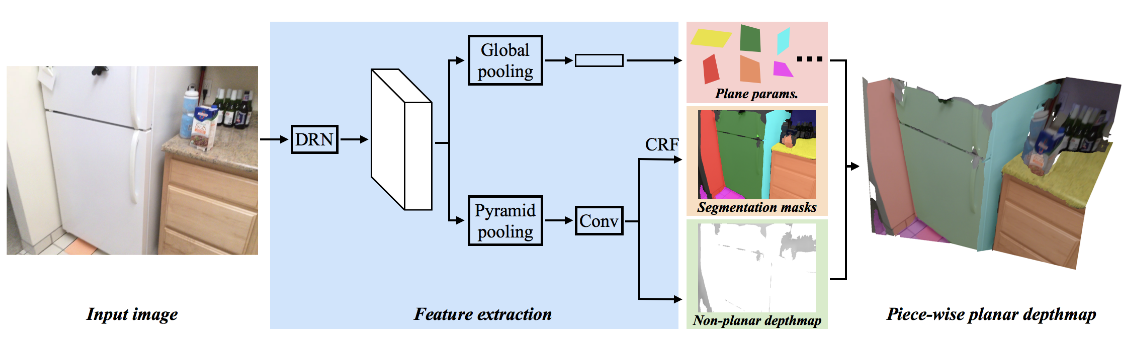
\includegraphics[width=\textwidth]{images/planenet.png}
    \caption[PlaneNet Architecture]{The PlaneNet Architecture. Taken from the respective paper~\cite[Figure~2]{Liu_Yang_Ceylan_Yumer_Furukawa_2018}.}
    \label{fig:planenet}
\end{figure}


The method implements a \textit{Dilated Residual Networks} (DRNs)~\cite{yu2017dilated} as a precursor for a total of three output branches.
These three branches predict
\begin{enumerate}
    \item A set of plane parameters,
    \item a set of corresponding segmentation masks, \textit{and}
    \item a non-planar depthmap,
\end{enumerate}
as portrayed in Figure~\ref{fig:planenet}. The DRN is followed by a global pooling, or a pyramid pooling step, depending on the prediction branch.
To obtain a set of plane parameters, the global pooling is followed by a fully connected layer, which produces $K$ parameter triples. $K$ corresponds to the number of
expected planes within a scene. \citeauthor{Liu_Yang_Ceylan_Yumer_Furukawa_2018}~\cite{Liu_Yang_Ceylan_Yumer_Furukawa_2018} use $K=10$ during their experiments.
A convolution layer is placed after the pyramid pooling the output of which is returned by the \textit{non-planar depthmap} branch.
An additional dense conditional random field (DCRF) is applied to obtain the segmentation masks.

\subsection{PlaneRecNet}
\label{subsec:bg-planerecnet}
PlaneRecNet~\cite{Xie_Shu_Rambach_Pagani_Stricker_2022} is a deep learning-based approach for piece-wise plane detection and reconstruction that takes RGB images
as input.
\begin{figure}[H]
    \centering
    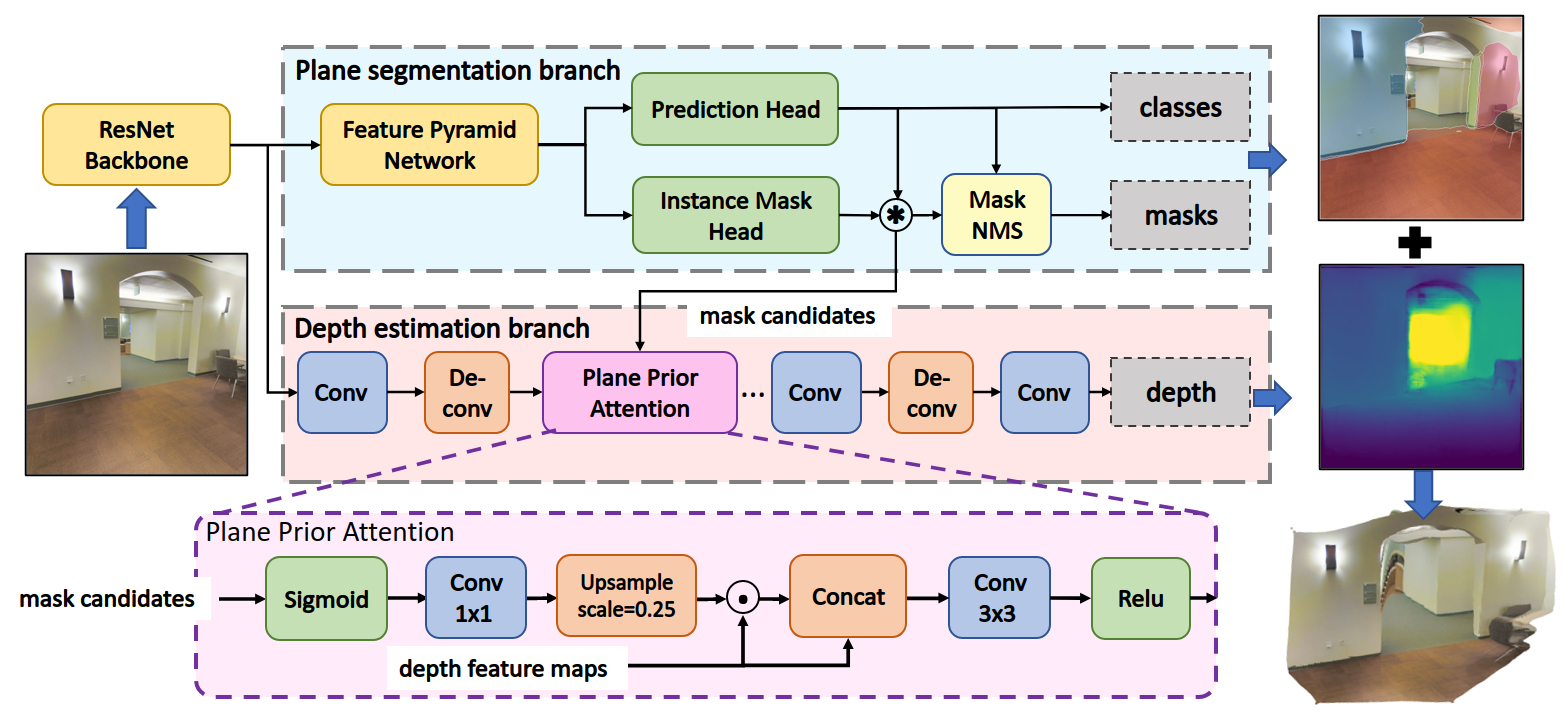
\includegraphics[width=\textwidth]{images/planerecnet.png}
    \caption[PlaneRecNet Architecture]{The PlaneRecNet Architecture. Taken from the respective paper~\cite[Figure~1]{Xie_Shu_Rambach_Pagani_Stricker_2022}}.
    \label{fig:planerecnet}
\end{figure}

The entire architecture of PlaneRecNet is portrayed in Figure~\ref{fig:planerecnet}.
The general approach of this method is to calculate plane parameters through principle component analysis (PCA) or RANSAC
after providing a precisely estimated depth.
This is achieved by implementing two separate branches, namely \textit{Plane segmentation}, and \textit{Depth estimation}.
Both branches obtain their input from a common precursor which is a \textit{ResNet}~\cite{He_Zhang_Ren_Sun_2015} backbone.
The \textit{Plane segmentation} branch is a lightweight configuration of SOLOV2~\cite{wang2020solov2} that has been modified to
fit the context of plane detection.
The \textit{Depth estimation} branch is a lightweight \textit{Feature Pyramid Network} (FPN)~\cite{Lin_Dollár_Girshick_He_Hariharan_Belongie_2017}.
Within the \textit{Depth estimation} branch, a so-called \textit{Plane Prior Attention} (PPA) module is used to introduce
the mask candidates from the \textit{Plane segmentation} branch into the depth estimation. The PPA module is based
on the \textit{Depth Attention Volume}~\cite{Huynh_Nguyen-Ha_Matas_Rahtu_Heikkila_2020}.

The estimated depth values and the segmentation masks, and classes, are then combined into a piecewise planar
scene reconstruction of the input image. No further refinement is implemented.

\subsection{PlaneRCNN}
\label{subsec:bg-planercnn}
RCNN~\cite{Liu_Kim_Gu_Furukawa_Kautz_2019} is a deep neural architecture that detects planar
regions and reconstructs a piecewise planar depth map from RGB-Images.

\begin{figure}[H]
    \centering
    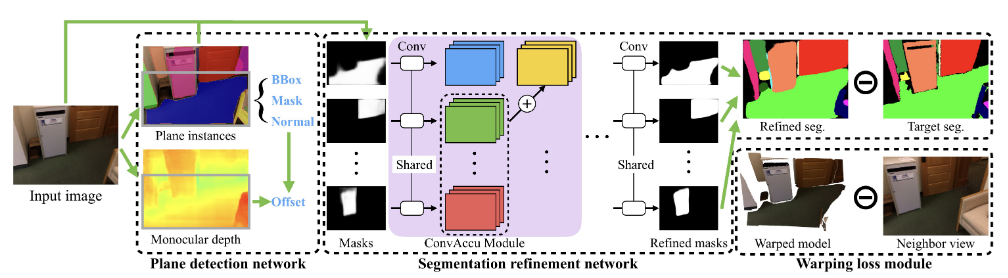
\includegraphics[width=\textwidth]{images/planercnn.png}
    \caption[PlaneRCNN Architecture]{The PlaneRCNN Architecture. Taken from the respective paper~\cite[Figure~2]{Liu_Kim_Gu_Furukawa_Kautz_2019}.}
    \label{fig:planercnn}
\end{figure}

The architecture of PlaneRCNN, as seen in Figure~\ref{fig:planercnn}, consists of three primary modules:
\begin{enumerate}
    \item The plane detection network,
    \item a segmentation refinement network, \textit{and}
    \item a warping loss module.
\end{enumerate}
The first module is built upon the semantic segmentation network MaskRCNN~\cite{he2017mask}. The module is modified to differentiate between "planar" and "non-planar"
object instances. In contrast to \textit{PlaneNet} (see Subsection~\ref{subsec:bg-planenet}), the number of planes to detect is not pre-determined. Moreover,
plane parameters and segmentation masks are calculated.

The second module, namely the \textit{segmentation refinement network}, refines the extracted segmentation masks obtained from the \textit{plane detection network}.
This is done by introducing non-locality into a U-Net~\cite{ronneberger2015u} by combining a convolution layer with an accumulation of feature volumes. The authors name this
particular step the \textit{ConvAccu} module~\cite[Section~3.2]{Liu_Kim_Gu_Furukawa_Kautz_2019}.

The \textit{warping loss module} implements a refinement step.  This module uses a second angle of the same view to ensure consistency. A view from 20 frames ahead is
projected into the current view to further refine the segmentation process. It is worth noting, that this is only performed during training to improve the accuracy.

\section{Datasets}
This section outlines a set of datasets popular in the evaluation of algorithms
in the field of plane detection. Table~\ref{tab:datasets} summarizes the key characteristics of each
dataset. The individual datasets are outlined in the following subsections.

\subsection{2D-3D-S}
\label{subsec:bg-stanford}
\textit{2D-3D-S}~\cite{2017arXiv170201105A} was recorded in three different buildings and divided into six distinct areas, including 272 different scenes. A detailed statistic of the included scene types can be found in Table~\ref{tab:stanfordStats}.
An individual scene has a complete unstructured point cloud and a list of annotated files representing semantically different objects that can be found therein.
The dataset includes a wide range of point cloud sizes, with a minimum of $8\cdot 10^4$ and a maximum of $7\cdot 10^6$
Furthermore, the average amount of points per scene is ${\sim}10^6$ with an average file size of ${\sim}34mb$.

\subsection{Leica}
\label{subsec:bg-Leica}
The Leica\footnote{\href{https://shop.leica-geosystems.com/de/leica-blk/blk360/dataset-downloads}{https://shop.leica-geosystems.com/de/leica-blk/blk360/dataset-downloads}}
dataset is a collection of 23 scans of outdoor environments.
Each scan consists of a dense unorganized point cloud which has been recorded by the \textit{Leica BLK360}
LiDAR Scanner\footnote{\href{https://shop.leica-geosystems.com/de/leica-blk/blk360}{https://shop.leica-geosystems.com/de/leica-blk/blk360}}.
The dataset is saved in \textit{ASTM E57}~\cite{Huber-2011-7211}, which is a general-purpose file format usually used for the
storage of 3D data, e.g., point clouds, laser scans or images.

\subsection{Kinect}
\label{subsec:bg-Kinect}
The \textit{Kinect}~\cite{Oehler_Stueckler_Welle_Schulz_Behnke_2011} dataset is a set of 30 organized point clouds. The recording was performed, as the
dataset's name suggests, with a Microsoft Kinect camera with a 640x480 resolution.
A ground truth that focuses on plane and cylinder segmentation is provided in addition to the point clouds.

\subsection{SYNPEB}
\label{subsec:bg-SYNPEB}
The \textit{SYNPEB} dataset was introduced by \citeauthor{schaefer19icra}~\cite{schaefer19icra} to improve upon the popular
\textit{SegComp} dataset. The synthetic dataset includes a 6x7x3m room with various geometric objects inside (see Figure~\ref{fig:SYNPEB}).
Moreover, a total of 40 scans from different views within the room are provided as organized point clouds with
a resolution of 500x500. Lastly, the provided ground truth represents a planar segmentation of the scene.

\begin{figure}[H]
    \centering
    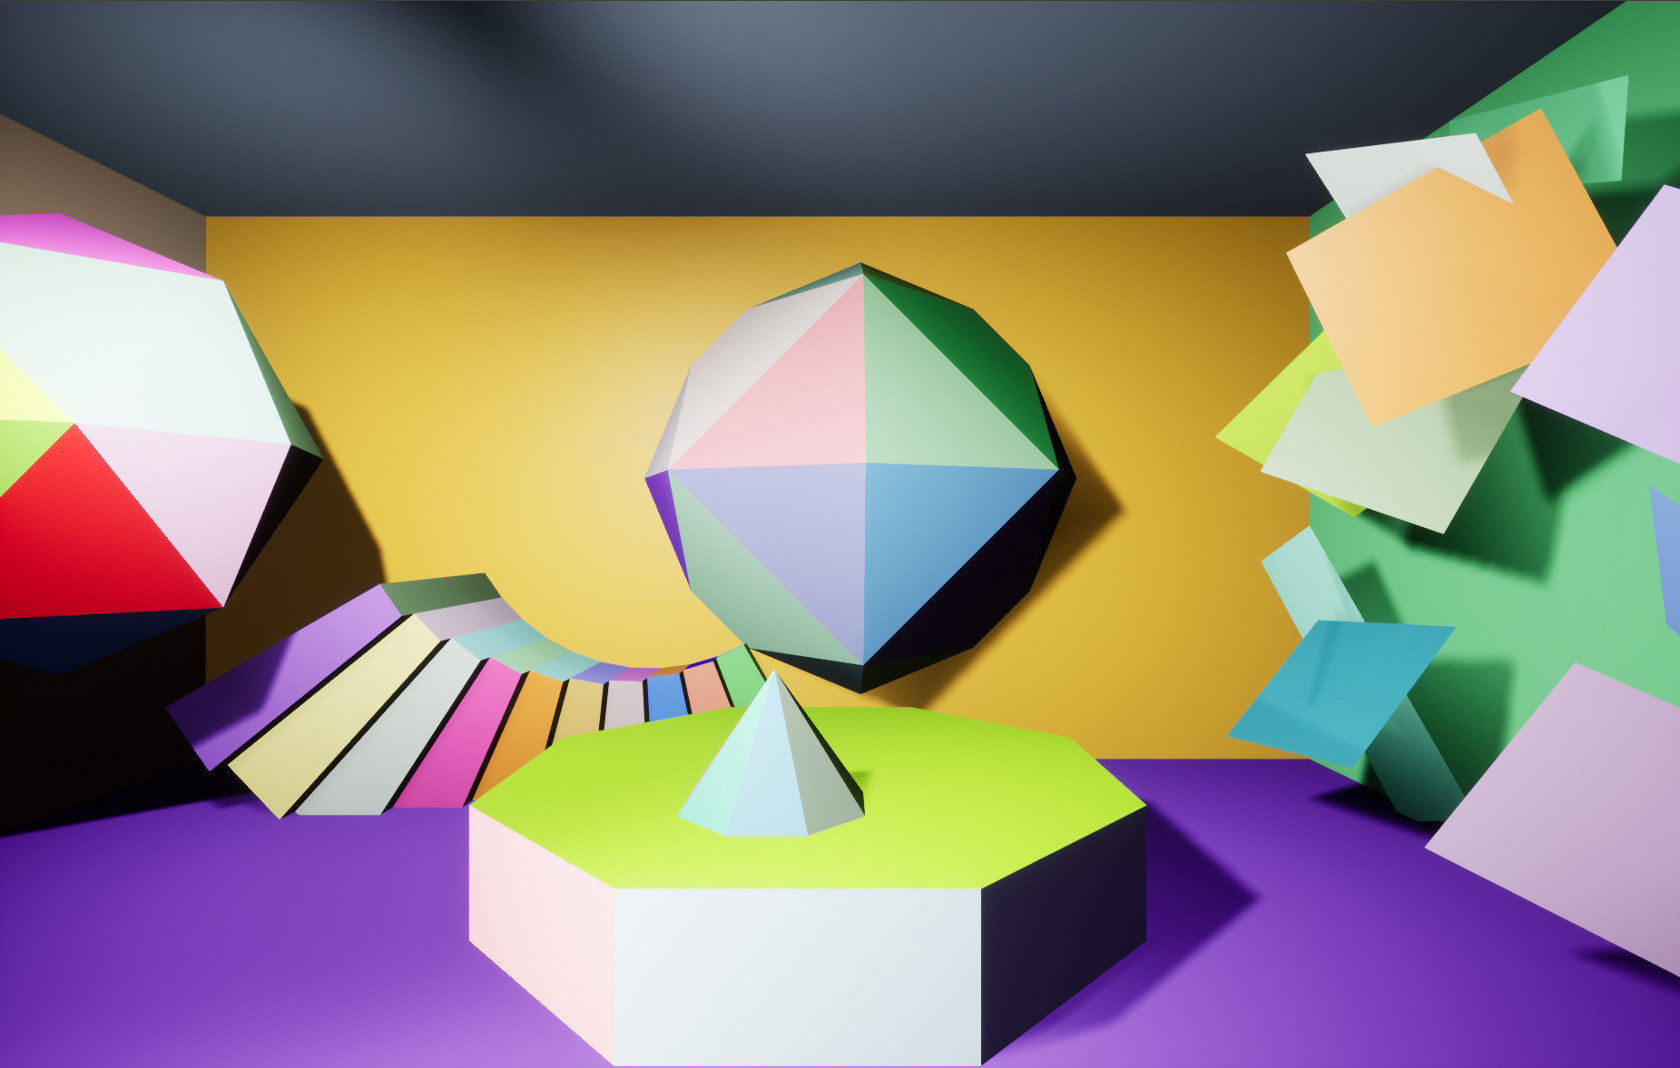
\includegraphics[width=\textwidth]{images/synpeb_room.jpg}
    \caption[SYNPEB]{The \textit{SYNPEB} room, taken from \href{http://synpeb.cs.uni-freiburg.de/}{http://synpeb.cs.uni-freiburg.de/}.}
    \label{fig:SYNPEB}
\end{figure}

\subsection{ARCO}
\label{subsec:bg-ARCO}
The \textit{ARCO}~\cite{Hidalgo-Paniagua_Vega-Rodriguez_Pavón_Ferruz_2015} dataset consists of 6 organized point clouds that have been recorded with a Microsoft Kinect camera.
All scenes show real indoor spaces, including a living room, a kitchen, a saloon, a hallway, furniture, and an ordinary room.
They are saved in the popular \textit{.pcd}\footnote{\href{http://pointclouds.org/documentation/tutorials/pcd\_file\_format}{http://pointclouds.org/documentation/tutorials/pcd\_file\_format}} file format.
We are not aware of the existence of a ground truth.

\subsection{SegComp}
\label{subsec:bg-segcomp}
The \textit{SegComp}~\cite{article} dataset
includes a collection of over 400 depth images, as well as a corresponding ground truth. Additionally, a complete
evaluation package is provided on the corresponding website\footnote{\href{http://www.eng.usf.edu/cvprg/range/seg-comp/SegComp.html}{http://www.eng.usf.edu/cvprg/range/seg-comp/SegComp.html}}.
The images are saved in their own file format, namely \textit{gt-seq}.

\subsection{NYU V2}
\label{subsec:bg-NYU}
The \textit{NYU-V2}~\cite{10.1007/978-3-642-33715-4_54} dataset is an improvement of the preceding version, namely \textit{NYU-V1}\footnote{\href{https://cs.nyu.edu/\~silberman/datasets/nyu\_depth\_v1.html}{https://cs.nyu.edu/\~silberman/datasets/nyu\_depth\_v1.html}}.
The dataset consists of 1449 RGB-D images, 464 scenes from 3 cities, and more than $400,000$ unlabeled frames.
A ground truth in form of labeled objects is provided, as well as a toolbox for arbitrary manipulation of data. Everything
was recorded with the Microsoft Kinect camera.

\subsection{ICL-NUIM}
\label{subsec:bg-ICL}
The \textit{ICL-NUIM}~\cite{Handa_Whelan_McDonald_Davison_2014} dataset was introduced for the benchmarking of RGB-D, VO and SLAM algorithms.
Eight scenes are included, which are comprised of a surface ground truth, depth images, and the trajectory of the camera.
The dataset includes a total of over 8000 images over these four scenes, whereas four have been recorded two
indoor environments, namely a living room, and an office.

\subsection{SUNRGB-D}
\label{subsec:bg-SUN}
The \textit{SUNRGB-D}~\cite{7298655} dataset is used for 3D object detection. The data is split into a training set and a testing set.
Over both sets, a total of over $13,000$ RGB-D images are included, with corresponding ground truths in form of 3D bounding boxes.
Furthermore, a toolbox is provided.
The dataset differentiates between 19 different objects, including, but not limited to: "wall", "door", "bookshelf", and "table".
More information can be found on the related website\footnote{\href{https://rgbd.cs.princeton.edu/challenge.html}{https://rgbd.cs.princeton.edu/challenge.html}}
under "Other Materials".

\subsection{TUM}
\label{subsec:bg-TUM}
The \textit{TUM}~\cite{sturm12iros} dataset was created for the evaluation of VO and Visual-SLAM systems.
A Microsoft Kinect sensor with a resolution of 640x480 is used to record a total of 39 scenes in indoor environments.
While the dataset is primarily focused on trajectories, organized point clouds are provided as well. A ground
truth trajectory is provided for each scene.
The dataset can be found on the project website \footnote{\href{https://vision.in.tum.de/data/datasets/rgbd-dataset/download}{.https://vision.in.tum.de/data/datasets/rgbd-dataset/download}}.

\section{Evaluation Metrics}
\label{sec:metrics}
Wenn man sachen segmentiert oder muster erkennen möchte usw. benutzt man oft zur evaluierung metriken, die die qualität der benutzten methode beschreiben.
Usual metrics are \textit{Precision, Recall} and the \textit{F1-Score}.
In general, \textit{Precision} describes how many of the results are relevant, i.e., the percentage of correctly calculated values(see Eq.~\ref{eq:prec}). \textit{Recall} describes the ratio of relevant results to all relevant data, i.e.
the likelihood of a result being relevant(see Eq.~\ref{eq:rec}). Lastly, the \textit{F1-Score} is the harmonic mean of the former two metrics (see Eq.~\ref{eq:f1}).

\begin{equation}
    Precision = \frac{\text{True Positive}}{\text{True Positive + False Positive}}
    \label{eq:prec}
\end{equation}

\begin{equation}
    Recall = \frac{\text{True Positive}}{\text{True Positive + False Negative}}
    \label{eq:rec}
\end{equation}

\begin{equation}
    \text{\textit{F1-Score}} = 2 \cdot\frac{Precision\cdot Recall}{Precision + Recall}
    \label{eq:f1}
\end{equation}



In the context of this work, we calculate \textit{Precision, Recall} and the \textit{F1-Score} as follows.
Required are the original point cloud $PC$, the corresponding list of ground truth planes $GT$ and the planes obtained from a plane detection algorithm $A$.
First, we regularize the $PC$ to reduce complexity and to avoid proximity bias, because of the inverse relationship
between distance to sensor and cloud density. This regularization is obtained through voxelization of the point cloud.
With this voxel grid, we can now calculate corresponding sets of voxels for each list of points that represent a plane.
In the next step, we compare our planes from $GT$ with $A$ to obtain a list of corresponding pairs of ground truth and found planes.
A ground truth plane $gt_i$ is marked as \textit{detected} if any plane from the list of found planes achieves a minimum voxel overlap of $50\%$.
With this list of correspondences, we calculate \textit{Precision, Recall} and the \textit{F1-Score}.

For a given ground truth plane $gt_j$ and a corresponding detected plane $a_k$ we can sort a given voxel $v_i$ into the categories
\textit{True Positive(TP), False Positive(FP) and False Negative(FN)} as follows.
$$v_i \in gt_j \land v_i \in a_k \Rightarrow v_{i} \in TP$$
$$v_i \in gt_j \land v_i \notin a_k \Rightarrow v_{i} \in FN$$
$$v_i \notin gt_j \land v_i \in a_k \Rightarrow v_{i} \in FP$$
% TODO not needed right? $$v_i \notin gt_j \land v_i \notin a_k \Rightarrow v_{i} \in TN$$  , True Negative(TN)} 

With those rules, we can calculate the Precision, Recall and F1 score like this:
$$Precision = \frac{|TP|}{|TP|+|FP|}$$
$$Recall = \frac{|TP|}{|TP|+|FN|}$$

\end{document}



